% one-figure manuscript written by fig_qc.py --tek-sekil-tex (trap T29)
\begin{figure}[!t]
\centering
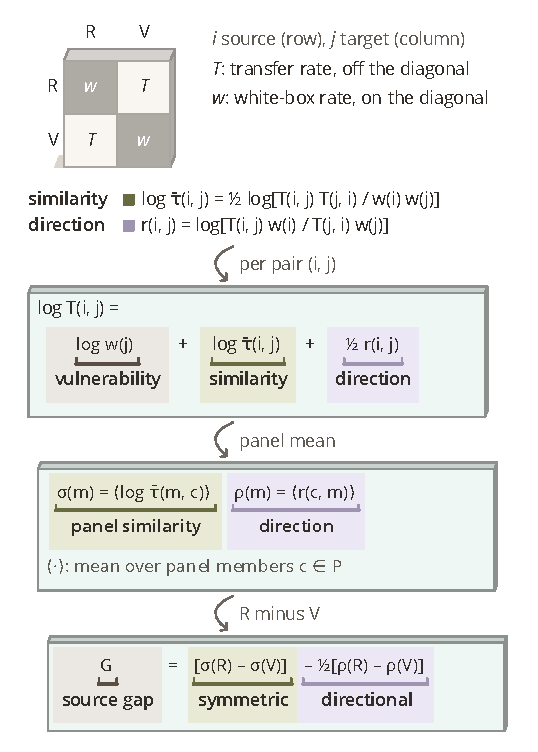
\includegraphics{fig3_decomposition_schematic}
\caption{\textbf{Decomposition used throughout, in three tiers.} Top to bottom, the arrows per pair (i, j), panel mean and R minus V mark three steps: the log transfer rate splits exactly into vulnerability, similarity and half a directional residual; panel averages give σ and ρ; the source gap G splits into symmetric and directional parts. Tiers recede with the aggregation level.}
\label{fig:fig3_decomposition_schematic}
\end{figure}
